%Master document for paper.
%Created MS 1/30

\documentclass[12pt]{article}
\usepackage{axodraw4j}
\usepackage[text={6.5in,9in},centering]{geometry}               % See geometry.pdf to learn the layout options. There are lots.
\geometry{letterpaper}                   % ... or a4paper or a5paper or ... 
%\geometry{landscape}                % Activate for for rotated page geometry
\usepackage[parfill]{parskip}    % Activate to begin paragraphs with an empty line rather than an indent
\usepackage{graphicx}
\usepackage{setspace}
\usepackage{color}
\usepackage{amssymb}
\usepackage{amsmath}
\usepackage{listings}
\usepackage{epstopdf}
\usepackage{epsfig}
% Psfig/TeX 
\def\PsfigVersion{1.9}
% dvips version
%
% All psfig/tex software, documentation, and related files
% in this distribution of psfig/tex are 
% Copyright 1987, 1988, 1991 Trevor J. Darrell
%
% Permission is granted for use and non-profit distribution of psfig/tex 
% providing that this notice is clearly maintained. The right to
% distribute any portion of psfig/tex for profit or as part of any commercial
% product is specifically reserved for the author(s) of that portion.
%
% *** Feel free to make local modifications of psfig as you wish,
% *** but DO NOT post any changed or modified versions of ``psfig''
% *** directly to the net. Send them to me and I'll try to incorporate
% *** them into future versions. If you want to take the psfig code 
% *** and make a new program (subject to the copyright above), distribute it, 
% *** (and maintain it) that's fine, just don't call it psfig.
%
% Bugs and improvements to trevor@media.mit.edu.
%
% Thanks to Greg Hager (GDH) and Ned Batchelder for their contributions
% to the original version of this project.
%
% Modified by J. Daniel Smith on 9 October 1990 to accept the
% %%BoundingBox: comment with or without a space after the colon.  Stole
% file reading code from Tom Rokicki's EPSF.TEX file (see below).
%
% More modifications by J. Daniel Smith on 29 March 1991 to allow the
% the included PostScript figure to be rotated.  The amount of
% rotation is specified by the "angle=" parameter of the \psfig command.
%
% Modified by Robert Russell on June 25, 1991 to allow users to specify
% .ps filenames which don't yet exist, provided they explicitly provide
% boundingbox information via the \psfig command. Note: This will only work
% if the "file=" parameter follows all four "bb???=" parameters in the
% command. This is due to the order in which psfig interprets these params.
%
%  3 Jul 1991	JDS	check if file already read in once
%  4 Sep 1991	JDS	fixed incorrect computation of rotated
%			bounding box
% 25 Sep 1991	GVR	expanded synopsis of \psfig
% 14 Oct 1991	JDS	\fbox code from LaTeX so \psdraft works with TeX
%			changed \typeout to \ps@typeout
% 17 Oct 1991	JDS	added \psscalefirst and \psrotatefirst
%

% From: gvr@cs.brown.edu (George V. Reilly)
%
% \psdraft	draws an outline box, but doesn't include the figure
%		in the DVI file.  Useful for previewing.
%
% \psfull	includes the figure in the DVI file (default).
%
% \psscalefirst width= or height= specifies the size of the figure
% 		before rotation.
% \psrotatefirst (default) width= or height= specifies the size of the
% 		 figure after rotation.  Asymetric figures will
% 		 appear to shrink.
%
% \psfigurepath#1	sets the path to search for the figure
%
% \psfig
% usage: \psfig{file=, figure=, height=, width=,
%			bbllx=, bblly=, bburx=, bbury=,
%			rheight=, rwidth=, clip=, angle=, silent=}
%
%	"file" is the filename.  If no path name is specified and the
%		file is not found in the current directory,
%		it will be looked for in directory \psfigurepath.
%	"figure" is a synonym for "file".
%	By default, the width and height of the figure are taken from
%		the BoundingBox of the figure.
%	If "width" is specified, the figure is scaled so that it has
%		the specified width.  Its height changes proportionately.
%	If "height" is specified, the figure is scaled so that it has
%		the specified height.  Its width changes proportionately.
%	If both "width" and "height" are specified, the figure is scaled
%		anamorphically.
%	"bbllx", "bblly", "bburx", and "bbury" control the PostScript
%		BoundingBox.  If these four values are specified
%               *before* the "file" option, the PSFIG will not try to
%               open the PostScript file.
%	"rheight" and "rwidth" are the reserved height and width
%		of the figure, i.e., how big TeX actually thinks
%		the figure is.  They default to "width" and "height".
%	The "clip" option ensures that no portion of the figure will
%		appear outside its BoundingBox.  "clip=" is a switch and
%		takes no value, but the `=' must be present.
%	The "angle" option specifies the angle of rotation (degrees, ccw).
%	The "silent" option makes \psfig work silently.
%

% check to see if macros already loaded in (maybe some other file says
% "\input psfig") ...
\ifx\undefined\psfig\else\endinput\fi

%
% from a suggestion by eijkhout@csrd.uiuc.edu to allow
% loading as a style file. Changed to avoid problems
% with amstex per suggestion by jbence@math.ucla.edu

\let\LaTeXAtSign=\@
\let\@=\relax
\edef\psfigRestoreAt{\catcode`\@=\number\catcode`@\relax}
%\edef\psfigRestoreAt{\catcode`@=\number\catcode`@\relax}
\catcode`\@=11\relax
\newwrite\@unused
\def\ps@typeout#1{{\let\protect\string\immediate\write\@unused{#1}}}
%\ps@typeout{psfig/tex \PsfigVersion}

%% Here's how you define your figure path.  Should be set up with null
%% default and a user useable definition.

\def\figurepath{./}
\def\psfigurepath#1{\edef\figurepath{#1}}

%
% @psdo control structure -- similar to Latex @for.
% I redefined these with different names so that psfig can
% be used with TeX as well as LaTeX, and so that it will not 
% be vunerable to future changes in LaTeX's internal
% control structure,
%
\def\@nnil{\@nil}
\def\@empty{}
\def\@psdonoop#1\@@#2#3{}
\def\@psdo#1:=#2\do#3{\edef\@psdotmp{#2}\ifx\@psdotmp\@empty \else
    \expandafter\@psdoloop#2,\@nil,\@nil\@@#1{#3}\fi}
\def\@psdoloop#1,#2,#3\@@#4#5{\def#4{#1}\ifx #4\@nnil \else
       #5\def#4{#2}\ifx #4\@nnil \else#5\@ipsdoloop #3\@@#4{#5}\fi\fi}
\def\@ipsdoloop#1,#2\@@#3#4{\def#3{#1}\ifx #3\@nnil 
       \let\@nextwhile=\@psdonoop \else
      #4\relax\let\@nextwhile=\@ipsdoloop\fi\@nextwhile#2\@@#3{#4}}
\def\@tpsdo#1:=#2\do#3{\xdef\@psdotmp{#2}\ifx\@psdotmp\@empty \else
    \@tpsdoloop#2\@nil\@nil\@@#1{#3}\fi}
\def\@tpsdoloop#1#2\@@#3#4{\def#3{#1}\ifx #3\@nnil 
       \let\@nextwhile=\@psdonoop \else
      #4\relax\let\@nextwhile=\@tpsdoloop\fi\@nextwhile#2\@@#3{#4}}
% 
% \fbox is defined in latex.tex; so if \fbox is undefined, assume that
% we are not in LaTeX.
% Perhaps this could be done better???
\ifx\undefined\fbox
% \fbox code from modified slightly from LaTeX
\newdimen\fboxrule
\newdimen\fboxsep
\newdimen\ps@tempdima
\newbox\ps@tempboxa
\fboxsep = 3pt
\fboxrule = .4pt
\long\def\fbox#1{\leavevmode\setbox\ps@tempboxa\hbox{#1}\ps@tempdima\fboxrule
    \advance\ps@tempdima \fboxsep \advance\ps@tempdima \dp\ps@tempboxa
   \hbox{\lower \ps@tempdima\hbox
  {\vbox{\hrule height \fboxrule
          \hbox{\vrule width \fboxrule \hskip\fboxsep
          \vbox{\vskip\fboxsep \box\ps@tempboxa\vskip\fboxsep}\hskip 
                 \fboxsep\vrule width \fboxrule}
                 \hrule height \fboxrule}}}}
\fi
%
%%%%%%%%%%%%%%%%%%%%%%%%%%%%%%%%%%%%%%%%%%%%%%%%%%%%%%%%%%%%%%%%%%%
% file reading stuff from epsf.tex
%   EPSF.TEX macro file:
%   Written by Tomas Rokicki of Radical Eye Software, 29 Mar 1989.
%   Revised by Don Knuth, 3 Jan 1990.
%   Revised by Tomas Rokicki to accept bounding boxes with no
%      space after the colon, 18 Jul 1990.
%   Portions modified/removed for use in PSFIG package by
%      J. Daniel Smith, 9 October 1990.
%
\newread\ps@stream
\newif\ifnot@eof       % continue looking for the bounding box?
\newif\if@noisy        % report what you're making?
\newif\if@atend        % %%BoundingBox: has (at end) specification
\newif\if@psfile       % does this look like a PostScript file?
%
% PostScript files should start with `%!'
%
{\catcode`\%=12\global\gdef\epsf@start{%!}}
\def\epsf@PS{PS}
%
\def\epsf@getbb#1{%
%
%   The first thing we need to do is to open the
%   PostScript file, if possible.
%
\openin\ps@stream=#1
\ifeof\ps@stream\ps@typeout{Error, File #1 not found}\else
%
%   Okay, we got it. Now we'll scan lines until we find one that doesn't
%   start with %. We're looking for the bounding box comment.
%
   {\not@eoftrue \chardef\other=12
    \def\do##1{\catcode`##1=\other}\dospecials \catcode`\ =10
    \loop
       \if@psfile
	  \read\ps@stream to \epsf@fileline
       \else{
	  \obeyspaces
          \read\ps@stream to \epsf@tmp\global\let\epsf@fileline\epsf@tmp}
       \fi
       \ifeof\ps@stream\not@eoffalse\else
%
%   Check the first line for `%!'.  Issue a warning message if its not
%   there, since the file might not be a PostScript file.
%
       \if@psfile\else
       \expandafter\epsf@test\epsf@fileline:. \\%
       \fi
%
%   We check to see if the first character is a % sign;
%   if so, we look further and stop only if the line begins with
%   `%%BoundingBox:' and the `(atend)' specification was not found.
%   That is, the only way to stop is when the end of file is reached,
%   or a `%%BoundingBox: llx lly urx ury' line is found.
%
          \expandafter\epsf@aux\epsf@fileline:. \\%
       \fi
   \ifnot@eof\repeat
   }\closein\ps@stream\fi}%
%
% This tests if the file we are reading looks like a PostScript file.
%
\long\def\epsf@test#1#2#3:#4\\{\def\epsf@testit{#1#2}
			\ifx\epsf@testit\epsf@start\else
\ps@typeout{Warning! File does not start with `\epsf@start'.  It may not be a PostScript file.}
			\fi
			\@psfiletrue} % don't test after 1st line
%
%   We still need to define the tricky \epsf@aux macro. This requires
%   a couple of magic constants for comparison purposes.
%
{\catcode`\%=12\global\let\epsf@percent=%\global\def\epsf@bblit{%BoundingBox}}
%
%
%   So we're ready to check for `%BoundingBox:' and to grab the
%   values if they are found.  We continue searching if `(at end)'
%   was found after the `%BoundingBox:'.
%
\long\def\epsf@aux#1#2:#3\\{\ifx#1\epsf@percent
   \def\epsf@testit{#2}\ifx\epsf@testit\epsf@bblit
	\@atendfalse
        \epsf@atend #3 . \\%
	\if@atend	
	   \if@verbose{
		\ps@typeout{psfig: found `(atend)'; continuing search}
	   }\fi
        \else
        \epsf@grab #3 . . . \\%
        \not@eoffalse
        \global\no@bbfalse
        \fi
   \fi\fi}%
%
%   Here we grab the values and stuff them in the appropriate definitions.
%
\def\epsf@grab #1 #2 #3 #4 #5\\{%
   \global\def\epsf@llx{#1}\ifx\epsf@llx\empty
      \epsf@grab #2 #3 #4 #5 .\\\else
   \global\def\epsf@lly{#2}%
   \global\def\epsf@urx{#3}\global\def\epsf@ury{#4}\fi}%
%
% Determine if the stuff following the %%BoundingBox is `(atend)'
% J. Daniel Smith.  Copied from \epsf@grab above.
%
\def\epsf@atendlit{(atend)} 
\def\epsf@atend #1 #2 #3\\{%
   \def\epsf@tmp{#1}\ifx\epsf@tmp\empty
      \epsf@atend #2 #3 .\\\else
   \ifx\epsf@tmp\epsf@atendlit\@atendtrue\fi\fi}


% End of file reading stuff from epsf.tex
%%%%%%%%%%%%%%%%%%%%%%%%%%%%%%%%%%%%%%%%%%%%%%%%%%%%%%%%%%%%%%%%%%%

%%%%%%%%%%%%%%%%%%%%%%%%%%%%%%%%%%%%%%%%%%%%%%%%%%%%%%%%%%%%%%%%%%%
% trigonometry stuff from "trig.tex"
\chardef\psletter = 11 % won't conflict with \begin{letter} now...
\chardef\other = 12

\newif \ifdebug %%% turn me on to see TeX hard at work ...
\newif\ifc@mpute %%% don't need to compute some values
\c@mputetrue % but assume that we do

\let\then = \relax
\def\r@dian{pt }
\let\r@dians = \r@dian
\let\dimensionless@nit = \r@dian
\let\dimensionless@nits = \dimensionless@nit
\def\internal@nit{sp }
\let\internal@nits = \internal@nit
\newif\ifstillc@nverging
\def \Mess@ge #1{\ifdebug \then \message {#1} \fi}

{ %%% Things that need abnormal catcodes %%%
	\catcode `\@ = \psletter
	\gdef \nodimen {\expandafter \n@dimen \the \dimen}
	\gdef \term #1 #2 #3%
	       {\edef \t@ {\the #1}%%% freeze parameter 1 (count, by value)
		\edef \t@@ {\expandafter \n@dimen \the #2\r@dian}%
				   %%% freeze parameter 2 (dimen, by value)
		\t@rm {\t@} {\t@@} {#3}%
	       }
	\gdef \t@rm #1 #2 #3%
	       {{%
		\count 0 = 0
		\dimen 0 = 1 \dimensionless@nit
		\dimen 2 = #2\relax
		\Mess@ge {Calculating term #1 of \nodimen 2}%
		\loop
		\ifnum	\count 0 < #1
		\then	\advance \count 0 by 1
			\Mess@ge {Iteration \the \count 0 \space}%
			\Multiply \dimen 0 by {\dimen 2}%
			\Mess@ge {After multiplication, term = \nodimen 0}%
			\Divide \dimen 0 by {\count 0}%
			\Mess@ge {After division, term = \nodimen 0}%
		\repeat
		\Mess@ge {Final value for term #1 of 
				\nodimen 2 \space is \nodimen 0}%
		\xdef \Term {#3 = \nodimen 0 \r@dians}%
		\aftergroup \Term
	       }}
	\catcode `\p = \other
	\catcode `\t = \other
	\gdef \n@dimen #1pt{#1} %%% throw away the ``pt''
}

\def \Divide #1by #2{\divide #1 by #2} %%% just a synonym

\def \Multiply #1by #2%%% allows division of a dimen by a dimen
       {{%%% should really freeze parameter 2 (dimen, passed by value)
	\count 0 = #1\relax
	\count 2 = #2\relax
	\count 4 = 65536
	\Mess@ge {Before scaling, count 0 = \the \count 0 \space and
			count 2 = \the \count 2}%
	\ifnum	\count 0 > 32767 %%% do our best to avoid overflow
	\then	\divide \count 0 by 4
		\divide \count 4 by 4
	\else	\ifnum	\count 0 < -32767
		\then	\divide \count 0 by 4
			\divide \count 4 by 4
		\else
		\fi
	\fi
	\ifnum	\count 2 > 32767 %%% while retaining reasonable accuracy
	\then	\divide \count 2 by 4
		\divide \count 4 by 4
	\else	\ifnum	\count 2 < -32767
		\then	\divide \count 2 by 4
			\divide \count 4 by 4
		\else
		\fi
	\fi
	\multiply \count 0 by \count 2
	\divide \count 0 by \count 4
	\xdef \product {#1 = \the \count 0 \internal@nits}%
	\aftergroup \product
       }}

\def\r@duce{\ifdim\dimen0 > 90\r@dian \then   % sin(x+90) = sin(180-x)
		\multiply\dimen0 by -1
		\advance\dimen0 by 180\r@dian
		\r@duce
	    \else \ifdim\dimen0 < -90\r@dian \then  % sin(-x) = sin(360+x)
		\advance\dimen0 by 360\r@dian
		\r@duce
		\fi
	    \fi}

\def\Sine#1%
       {{%
	\dimen 0 = #1 \r@dian
	\r@duce
	\ifdim\dimen0 = -90\r@dian \then
	   \dimen4 = -1\r@dian
	   \c@mputefalse
	\fi
	\ifdim\dimen0 = 90\r@dian \then
	   \dimen4 = 1\r@dian
	   \c@mputefalse
	\fi
	\ifdim\dimen0 = 0\r@dian \then
	   \dimen4 = 0\r@dian
	   \c@mputefalse
	\fi
%
	\ifc@mpute \then
        	% convert degrees to radians
		\divide\dimen0 by 180
		\dimen0=3.141592654\dimen0
%
		\dimen 2 = 3.1415926535897963\r@dian %%% a well-known constant
		\divide\dimen 2 by 2 %%% we only deal with -pi/2 : pi/2
		\Mess@ge {Sin: calculating Sin of \nodimen 0}%
		\count 0 = 1 %%% see power-series expansion for sine
		\dimen 2 = 1 \r@dian %%% ditto
		\dimen 4 = 0 \r@dian %%% ditto
		\loop
			\ifnum	\dimen 2 = 0 %%% then we've done
			\then	\stillc@nvergingfalse 
			\else	\stillc@nvergingtrue
			\fi
			\ifstillc@nverging %%% then calculate next term
			\then	\term {\count 0} {\dimen 0} {\dimen 2}%
				\advance \count 0 by 2
				\count 2 = \count 0
				\divide \count 2 by 2
				\ifodd	\count 2 %%% signs alternate
				\then	\advance \dimen 4 by \dimen 2
				\else	\advance \dimen 4 by -\dimen 2
				\fi
		\repeat
	\fi		
			\xdef \sine {\nodimen 4}%
       }}

% Now the Cosine can be calculated easily by calling \Sine
\def\Cosine#1{\ifx\sine\UnDefined\edef\Savesine{\relax}\else
		             \edef\Savesine{\sine}\fi
	{\dimen0=#1\r@dian\advance\dimen0 by 90\r@dian
	 \Sine{\nodimen 0}
	 \xdef\cosine{\sine}
	 \xdef\sine{\Savesine}}}	      
% end of trig stuff
%%%%%%%%%%%%%%%%%%%%%%%%%%%%%%%%%%%%%%%%%%%%%%%%%%%%%%%%%%%%%%%%%%%%

\def\psdraft{
	\def\@psdraft{0}
	%\ps@typeout{draft level now is \@psdraft \space . }
}
\def\psfull{
	\def\@psdraft{100}
	%\ps@typeout{draft level now is \@psdraft \space . }
}

\psfull

\newif\if@scalefirst
\def\psscalefirst{\@scalefirsttrue}
\def\psrotatefirst{\@scalefirstfalse}
\psrotatefirst

\newif\if@draftbox
\def\psnodraftbox{
	\@draftboxfalse
}
\def\psdraftbox{
	\@draftboxtrue
}
\@draftboxtrue

\newif\if@prologfile
\newif\if@postlogfile
\def\pssilent{
	\@noisyfalse
}
\def\psnoisy{
	\@noisytrue
}
\psnoisy
%%% These are for the option list.
%%% A specification of the form a = b maps to calling \@p@@sa{b}
\newif\if@bbllx
\newif\if@bblly
\newif\if@bburx
\newif\if@bbury
\newif\if@height
\newif\if@width
\newif\if@rheight
\newif\if@rwidth
\newif\if@angle
\newif\if@clip
\newif\if@verbose
\def\@p@@sclip#1{\@cliptrue}


\newif\if@decmpr

%%% GDH 7/26/87 -- changed so that it first looks in the local directory,
%%% then in a specified global directory for the ps file.
%%% RPR 6/25/91 -- changed so that it defaults to user-supplied name if
%%% boundingbox info is specified, assuming graphic will be created by
%%% print time.
%%% TJD 10/19/91 -- added bbfile vs. file distinction, and @decmpr flag

\def\@p@@sfigure#1{\def\@p@sfile{null}\def\@p@sbbfile{null}
	        \openin1=#1.bb
		\ifeof1\closein1
	        	\openin1=\figurepath#1.bb
			\ifeof1\closein1
			        \openin1=#1
				\ifeof1\closein1%
				       \openin1=\figurepath#1
					\ifeof1
					   \ps@typeout{Error, File #1 not found}
						\if@bbllx\if@bblly
				   		\if@bburx\if@bbury
			      				\def\@p@sfile{#1}%
			      				\def\@p@sbbfile{#1}%
							\@decmprfalse
				  	   	\fi\fi\fi\fi
					\else\closein1
				    		\def\@p@sfile{\figurepath#1}%
				    		\def\@p@sbbfile{\figurepath#1}%
						\@decmprfalse
	                       		\fi%
			 	\else\closein1%
					\def\@p@sfile{#1}
					\def\@p@sbbfile{#1}
					\@decmprfalse
			 	\fi
			\else
				\def\@p@sfile{\figurepath#1}
				\def\@p@sbbfile{\figurepath#1.bb}
				\@decmprtrue
			\fi
		\else
			\def\@p@sfile{#1}
			\def\@p@sbbfile{#1.bb}
			\@decmprtrue
		\fi}

\def\@p@@sfile#1{\@p@@sfigure{#1}}

\def\@p@@sbbllx#1{
		%\ps@typeout{bbllx is #1}
		\@bbllxtrue
		\dimen100=#1
		\edef\@p@sbbllx{\number\dimen100}
}
\def\@p@@sbblly#1{
		%\ps@typeout{bblly is #1}
		\@bbllytrue
		\dimen100=#1
		\edef\@p@sbblly{\number\dimen100}
}
\def\@p@@sbburx#1{
		%\ps@typeout{bburx is #1}
		\@bburxtrue
		\dimen100=#1
		\edef\@p@sbburx{\number\dimen100}
}
\def\@p@@sbbury#1{
		%\ps@typeout{bbury is #1}
		\@bburytrue
		\dimen100=#1
		\edef\@p@sbbury{\number\dimen100}
}
\def\@p@@sheight#1{
		\@heighttrue
		\dimen100=#1
   		\edef\@p@sheight{\number\dimen100}
		%\ps@typeout{Height is \@p@sheight}
}
\def\@p@@swidth#1{
		%\ps@typeout{Width is #1}
		\@widthtrue
		\dimen100=#1
		\edef\@p@swidth{\number\dimen100}
}
\def\@p@@srheight#1{
		%\ps@typeout{Reserved height is #1}
		\@rheighttrue
		\dimen100=#1
		\edef\@p@srheight{\number\dimen100}
}
\def\@p@@srwidth#1{
		%\ps@typeout{Reserved width is #1}
		\@rwidthtrue
		\dimen100=#1
		\edef\@p@srwidth{\number\dimen100}
}
\def\@p@@sangle#1{
		%\ps@typeout{Rotation is #1}
		\@angletrue
%		\dimen100=#1
		\edef\@p@sangle{#1} %\number\dimen100}
}
\def\@p@@ssilent#1{ 
		\@verbosefalse
}
\def\@p@@sprolog#1{\@prologfiletrue\def\@prologfileval{#1}}
\def\@p@@spostlog#1{\@postlogfiletrue\def\@postlogfileval{#1}}
\def\@cs@name#1{\csname #1\endcsname}
\def\@setparms#1=#2,{\@cs@name{@p@@s#1}{#2}}
%
% initialize the defaults (size the size of the figure)
%
\def\ps@init@parms{
		\@bbllxfalse \@bbllyfalse
		\@bburxfalse \@bburyfalse
		\@heightfalse \@widthfalse
		\@rheightfalse \@rwidthfalse
		\def\@p@sbbllx{}\def\@p@sbblly{}
		\def\@p@sbburx{}\def\@p@sbbury{}
		\def\@p@sheight{}\def\@p@swidth{}
		\def\@p@srheight{}\def\@p@srwidth{}
		\def\@p@sangle{0}
		\def\@p@sfile{} \def\@p@sbbfile{}
		\def\@p@scost{10}
		\def\@sc{}
		\@prologfilefalse
		\@postlogfilefalse
		\@clipfalse
		\if@noisy
			\@verbosetrue
		\else
			\@verbosefalse
		\fi
}
%
% Go through the options setting things up.
%
\def\parse@ps@parms#1{
	 	\@psdo\@psfiga:=#1\do
		   {\expandafter\@setparms\@psfiga,}}
%
% Compute bb height and width
%
\newif\ifno@bb
\def\bb@missing{
	\if@verbose{
		\ps@typeout{psfig: searching \@p@sbbfile \space  for bounding box}
	}\fi
	\no@bbtrue
	\epsf@getbb{\@p@sbbfile}
        \ifno@bb \else \bb@cull\epsf@llx\epsf@lly\epsf@urx\epsf@ury\fi
}	
\def\bb@cull#1#2#3#4{
	\dimen100=#1 bp\edef\@p@sbbllx{\number\dimen100}
	\dimen100=#2 bp\edef\@p@sbblly{\number\dimen100}
	\dimen100=#3 bp\edef\@p@sbburx{\number\dimen100}
	\dimen100=#4 bp\edef\@p@sbbury{\number\dimen100}
	\no@bbfalse
}
% rotate point (#1,#2) about (0,0).
% The sine and cosine of the angle are already stored in \sine and
% \cosine.  The result is placed in (\p@intvaluex, \p@intvaluey).
\newdimen\p@intvaluex
\newdimen\p@intvaluey
\def\rotate@#1#2{{\dimen0=#1 sp\dimen1=#2 sp
%            	calculate x' = x \cos\theta - y \sin\theta
		  \global\p@intvaluex=\cosine\dimen0
		  \dimen3=\sine\dimen1
		  \global\advance\p@intvaluex by -\dimen3
% 		calculate y' = x \sin\theta + y \cos\theta
		  \global\p@intvaluey=\sine\dimen0
		  \dimen3=\cosine\dimen1
		  \global\advance\p@intvaluey by \dimen3
		  }}
\def\compute@bb{
		\no@bbfalse
		\if@bbllx \else \no@bbtrue \fi
		\if@bblly \else \no@bbtrue \fi
		\if@bburx \else \no@bbtrue \fi
		\if@bbury \else \no@bbtrue \fi
		\ifno@bb \bb@missing \fi
		\ifno@bb \ps@typeout{FATAL ERROR: no bb supplied or found}
			\no-bb-error
		\fi
		%
%\ps@typeout{BB: \@p@sbbllx, \@p@sbblly, \@p@sbburx, \@p@sbbury} 
%
% store height/width of original (unrotated) bounding box
		\count203=\@p@sbburx
		\count204=\@p@sbbury
		\advance\count203 by -\@p@sbbllx
		\advance\count204 by -\@p@sbblly
		\edef\ps@bbw{\number\count203}
		\edef\ps@bbh{\number\count204}
		%\ps@typeout{ psbbh = \ps@bbh, psbbw = \ps@bbw }
		\if@angle 
			\Sine{\@p@sangle}\Cosine{\@p@sangle}
	        	{\dimen100=\maxdimen\xdef\r@p@sbbllx{\number\dimen100}
					    \xdef\r@p@sbblly{\number\dimen100}
			                    \xdef\r@p@sbburx{-\number\dimen100}
					    \xdef\r@p@sbbury{-\number\dimen100}}
%
% Need to rotate all four points and take the X-Y extremes of the new
% points as the new bounding box.
                        \def\minmaxtest{
			   \ifnum\number\p@intvaluex<\r@p@sbbllx
			      \xdef\r@p@sbbllx{\number\p@intvaluex}\fi
			   \ifnum\number\p@intvaluex>\r@p@sbburx
			      \xdef\r@p@sbburx{\number\p@intvaluex}\fi
			   \ifnum\number\p@intvaluey<\r@p@sbblly
			      \xdef\r@p@sbblly{\number\p@intvaluey}\fi
			   \ifnum\number\p@intvaluey>\r@p@sbbury
			      \xdef\r@p@sbbury{\number\p@intvaluey}\fi
			   }
%			lower left
			\rotate@{\@p@sbbllx}{\@p@sbblly}
			\minmaxtest
%			upper left
			\rotate@{\@p@sbbllx}{\@p@sbbury}
			\minmaxtest
%			lower right
			\rotate@{\@p@sbburx}{\@p@sbblly}
			\minmaxtest
%			upper right
			\rotate@{\@p@sbburx}{\@p@sbbury}
			\minmaxtest
			\edef\@p@sbbllx{\r@p@sbbllx}\edef\@p@sbblly{\r@p@sbblly}
			\edef\@p@sbburx{\r@p@sbburx}\edef\@p@sbbury{\r@p@sbbury}
%\ps@typeout{rotated BB: \r@p@sbbllx, \r@p@sbblly, \r@p@sbburx, \r@p@sbbury}
		\fi
		\count203=\@p@sbburx
		\count204=\@p@sbbury
		\advance\count203 by -\@p@sbbllx
		\advance\count204 by -\@p@sbblly
		\edef\@bbw{\number\count203}
		\edef\@bbh{\number\count204}
		%\ps@typeout{ bbh = \@bbh, bbw = \@bbw }
}
%
% \in@hundreds performs #1 * (#2 / #3) correct to the hundreds,
%	then leaves the result in @result
%
\def\in@hundreds#1#2#3{\count240=#2 \count241=#3
		     \count100=\count240	% 100 is first digit #2/#3
		     \divide\count100 by \count241
		     \count101=\count100
		     \multiply\count101 by \count241
		     \advance\count240 by -\count101
		     \multiply\count240 by 10
		     \count101=\count240	%101 is second digit of #2/#3
		     \divide\count101 by \count241
		     \count102=\count101
		     \multiply\count102 by \count241
		     \advance\count240 by -\count102
		     \multiply\count240 by 10
		     \count102=\count240	% 102 is the third digit
		     \divide\count102 by \count241
		     \count200=#1\count205=0
		     \count201=\count200
			\multiply\count201 by \count100
		 	\advance\count205 by \count201
		     \count201=\count200
			\divide\count201 by 10
			\multiply\count201 by \count101
			\advance\count205 by \count201
			%
		     \count201=\count200
			\divide\count201 by 100
			\multiply\count201 by \count102
			\advance\count205 by \count201
			%
		     \edef\@result{\number\count205}
}
\def\compute@wfromh{
		% computing : width = height * (bbw / bbh)
		\in@hundreds{\@p@sheight}{\@bbw}{\@bbh}
		%\ps@typeout{ \@p@sheight * \@bbw / \@bbh, = \@result }
		\edef\@p@swidth{\@result}
		%\ps@typeout{w from h: width is \@p@swidth}
}
\def\compute@hfromw{
		% computing : height = width * (bbh / bbw)
	        \in@hundreds{\@p@swidth}{\@bbh}{\@bbw}
		%\ps@typeout{ \@p@swidth * \@bbh / \@bbw = \@result }
		\edef\@p@sheight{\@result}
		%\ps@typeout{h from w : height is \@p@sheight}
}
\def\compute@handw{
		\if@height 
			\if@width
			\else
				\compute@wfromh
			\fi
		\else 
			\if@width
				\compute@hfromw
			\else
				\edef\@p@sheight{\@bbh}
				\edef\@p@swidth{\@bbw}
			\fi
		\fi
}
\def\compute@resv{
		\if@rheight \else \edef\@p@srheight{\@p@sheight} \fi
		\if@rwidth \else \edef\@p@srwidth{\@p@swidth} \fi
		%\ps@typeout{rheight = \@p@srheight, rwidth = \@p@srwidth}
}
%		
% Compute any missing values
\def\compute@sizes{
	\compute@bb
	\if@scalefirst\if@angle
% at this point the bounding box has been adjsuted correctly for
% rotation.  PSFIG does all of its scaling using \@bbh and \@bbw.  If
% a width= or height= was specified along with \psscalefirst, then the
% width=/height= value needs to be adjusted to match the new (rotated)
% bounding box size (specifed in \@bbw and \@bbh).
%    \ps@bbw       width=
%    -------  =  ---------- 
%    \@bbw       new width=
% so `new width=' = (width= * \@bbw) / \ps@bbw; where \ps@bbw is the
% width of the original (unrotated) bounding box.
	\if@width
	   \in@hundreds{\@p@swidth}{\@bbw}{\ps@bbw}
	   \edef\@p@swidth{\@result}
	\fi
	\if@height
	   \in@hundreds{\@p@sheight}{\@bbh}{\ps@bbh}
	   \edef\@p@sheight{\@result}
	\fi
	\fi\fi
	\compute@handw
	\compute@resv}

%
% \psfig
% usage : \psfig{file=, height=, width=, bbllx=, bblly=, bburx=, bbury=,
%			rheight=, rwidth=, clip=}
%
% "clip=" is a switch and takes no value, but the `=' must be present.
\def\psfig#1{\vbox {
	% do a zero width hard space so that a single
	% \psfig in a centering enviornment will behave nicely
	%{\setbox0=\hbox{\ }\ \hskip-\wd0}
	%
	\ps@init@parms
	\parse@ps@parms{#1}
	\compute@sizes
	%
	\ifnum\@p@scost<\@psdraft{
		%
		\special{ps::[begin] 	\@p@swidth \space \@p@sheight \space
				\@p@sbbllx \space \@p@sbblly \space
				\@p@sbburx \space \@p@sbbury \space
				startTexFig \space }
		\if@angle
			\special {ps:: \@p@sangle \space rotate \space} 
		\fi
		\if@clip{
			\if@verbose{
				\ps@typeout{(clip)}
			}\fi
			\special{ps:: doclip \space }
		}\fi
		\if@prologfile
		    \special{ps: plotfile \@prologfileval \space } \fi
		\if@decmpr{
			\if@verbose{
				\ps@typeout{psfig: including \@p@sfile.Z \space }
			}\fi
			\special{ps: plotfile "`zcat \@p@sfile.Z" \space }
		}\else{
			\if@verbose{
				\ps@typeout{psfig: including \@p@sfile \space }
			}\fi
			\special{ps: plotfile \@p@sfile \space }
		}\fi
		\if@postlogfile
		    \special{ps: plotfile \@postlogfileval \space } \fi
		\special{ps::[end] endTexFig \space }
		% Create the vbox to reserve the space for the figure.
		\vbox to \@p@srheight sp{
		% 1/92 TJD Changed from "true sp" to "sp" for magnification.
			\hbox to \@p@srwidth sp{
				\hss
			}
		\vss
		}
	}\else{
		% draft figure, just reserve the space and print the
		% path name.
		\if@draftbox{		
			% Verbose draft: print file name in box
			\hbox{\frame{\vbox to \@p@srheight sp{
			\vss
			\hbox to \@p@srwidth sp{ \hss \@p@sfile \hss }
			\vss
			}}}
		}\else{
			% Non-verbose draft
			\vbox to \@p@srheight sp{
			\vss
			\hbox to \@p@srwidth sp{\hss}
			\vss
			}
		}\fi	



	}\fi
}}
\psfigRestoreAt
\let\@=\LaTeXAtSign





\DeclareGraphicsRule{.tif}{png}{.png}{`convert #1 `dirname #1`/`basename #1 .tif`.png}
\usepackage{cite}
\usepackage{fancyheadings}


\begin{document}

\pagestyle{fancy}

\begin{small}
\lhead{\bfseries Maximilian Swiatlowski} 
\chead{} 
\rhead{\bfseries \today} 
\renewcommand{\headrulewidth}{0.1pt} 
\renewcommand{\footrulewidth}{0.1pt} 
\end{small}

\begin{center}
\begin{LARGE}
\bfseries Measurement of Weak Coupling Constant blahblah
\end{LARGE}
\end{center}

%Introduction body
%Created MS 1-30

\section{Introduction}\label{introduction}

The muon, a fundamental particle produced in the upper atmosphere as a
secondary product of cosmic ray collisions, was originally discovered
in 1936 \cite{}. It decays via the weak interaction with a mean decay
lifetime of $2.2 \mu s$, longer than every known particle other than
the neutron \cite{}. With muons comprising $80$\% of cosmic ray flux at
sea level, the muon is a good candidate for the study of the weak
force \cite{}.

Our experiment consists of two main components: the muon lifetime
measurement and the muon mass measurement. In section 2,
\emph{Background}, we introduce the theoretical basis for these
measurement as well as that of muon creation and decay. We describe
the experimental setup which consists of a system of three
scintillators and photomultiplier tubes (PMTs) in \emph{Setup}. Using
this system, the cosmic ray muons passing through the scintillators
and their decay products can be detected along with their enegy
(\emph{Procedure}). The muon lifetime and mass results are presented in
\emph{Results} and \emph{Discussion} with the relevant statistical
analysis of data, and compared to previous experimentally established
values. Finally, we use the muon mass and lifetime values to calculate
the weak force coupling constant, $g_w$.


%Background body
%Created MB 04-12

\section{Background}\label{background}

The $^4$He atom is one of the very simple and symmetrical systems
among the elements, with a filled innermost electron shell and no
overall electric or magnetic moment or angular momentum to the atom
\cite{atkins}. Due to the symmetric nature of helium atoms, the
interaction between them is very weak, and $^4$He liquifies at an
extremely low temperature of $4.21$ K. However, a more interesting
transition occurs at $2.17$ K, at which point liquid helium takes on
several unique properties. Below this temperature, termed the
$\lambda$ point, $^4$He\footnote{Although the isotope $^3$He is also
  capable of producing these effects, the transition temperature is
  much lower at $3\times 10^{-3}$ K and is unreachable with the
  cryogenic technology available to us. Thus, in the remainder of the
  paper, the isotope $^4$He is implied unless stated otherwise.}
acquires extremely high thermal conductivity, negligible viscocity,
and the ability to propagate temperature waves(second sound); in
addition, there is a $\lambda$-shaped discontinuity at the transition
in the heat capacity of liquid helium, which is how the $\lambda$
point acquires its name. To distinguish the two phases of liquid
helium, the liquid is referred to as helium I above the lambda point
and helium II below the lambda point (BLAHHH). The investigation of
the properties of helium II mentioned above will be the focus of this
paper.

\subsection{The Two-Fluid Model}

A key model explaining the unusual properties of He II was proposed by
Landau in 1941 as the two-fluid model \cite{landau}. In this theory,
the liquid below the $\lambda$-point can be viewed as being composed
of two noninteracting fluids: a superfluid component with density
$\rho_s$ and a normal component with density $\rho_n$, such that the
total density $\rho$ is given as the sum of the two components:
\begin{equation}
\rho = \rho_s + \rho_n
\end{equation}

and the total current density of He II is given by
\begin{equation}
\mathbf{j} = \rho_s\mathbf{v_s} + \rho_n\mathbf{v_n}
\end{equation}

where $\mathbf{v_s}$ and $\mathbf{v_n}$ are the velocities of the
superfluid and normal fluid, respectively \cite{tilley}. Then, the
behavior of the fluid can be understood in terms of the different
characteristic of the two components: while the normal fluid acts
according to the regular laws of fluid mechanics and satisfies the
Navier-Stokes equation, the superfluid has zero entropy and flows with
zero viscocity. Furthermore, it is important to note that the two
components are non-interacting, that is, there is no transfer of
momentum between the two fluids, and most importantly that they are
not physically distinct and cannot be separated \cite{tilley}.

With the incorporation of theories of Bose-Einstein condensates into
Landau's theory, further understanding of the fluid is possible. The
superfluid can be viewed as an interacting Bose-Einstein condensate
system, occupying a single macroscopic quantum state, whereas the
normal fluid consists the excitations (photons and rotons) of the
superfluid. As temperature decreases from $2.17$ to $0$ K, the
fraction of superfluid increases, from $0$ at the $\lambda$-point to
unity at absolute zero, as the excitations decrease to zero.

\begin{figure}[ht]
\begin{center}
%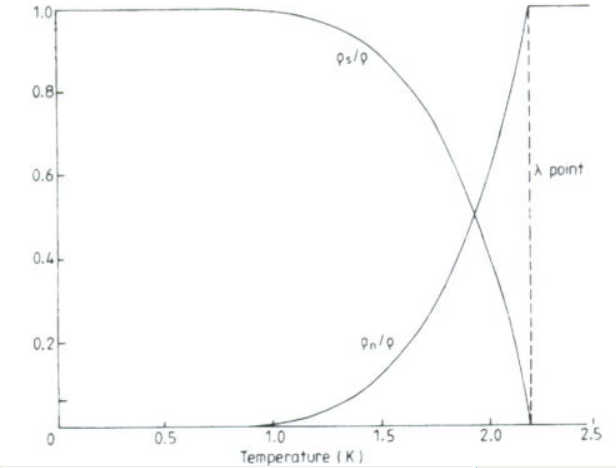
\includegraphics{./figures/twofluid.eps} WHY NOT WORKINGGGGGGG
%\{./figures/twofluid.eps}
\caption{\small{Relative fractions $\rho_s/\rho$ and $\rho_n/\rho$ of
    the superfluid and normal components in He II.}}
\label{figure:twofluid}
\end{center}
\end{figure}



\subsection{Second Sound}

The thermal conductivity of He II is very high, and tends to infinity
for small heat currents \cite{tilley}. This makes the fluid intolerant
to temperature gradients. This property explains the visually
noticeable transition from He I to He II with descreasing temperature:
while in He I, there is a lot of bubbling, as the temperature passes
the $\lambda$-point, the bubbling ceases immediately, since a
temperature gradient large enough cannot be established in order for a
bubble to form \cite{tilley}.

Interestingly, the superfluid fraction cannot transfer heat, but is
able to balance temperature gradients not through convection and
BLAHHOTHERTHING but through an exchange of the relative concentrations
of the two componenets $\rho_n$ and $\rho_s$. As seen in FIGURE
TWOFLUID, at lower temperatures the fraction of superfluid increases.

The relationship between velocity of second sound, $u_2$, and the
relative fractions of the fluids was derived analytically by Landau
and is given by

\begin{equation}
u_2^2 = \frac{\rho_s}{\rho_n}\frac{T S^2}{C}
\end{equation}

where $S$ and $C$ are the entropy and heat capacity per gram of the
liquid and can be measured experimentally \cite{atkins}. 

\subsection{Heat Capacity}


\section{Instrumentation}
\label{instrumentation}

In order to detect muon and electron events, signals from scintillators are correlated and matched against an expected pattern. The next section (\ref{procedure}) will discuss how these are used to generate lifetimes; here, we focus on describing the apparatus and problems associated with it.

\subsection{Scintillators}
\label{scintillators}

The scintillator consists of polystyrene ($\mathrm{C}_{8}\mathrm{H}_{9}$, with density $1.08 \pm .09 \frac{\mathrm{g}}{\mathrm{cm}^{3}}$) doped with a phosphorous material, p-terphenyl. When ionizing radiation passes through the material a light pulse is emitted. The light flash is detected by the photomultiplier tubes placed at the ends of the scintillator. The photomultiplier uses a high voltage (on the order of 1000 V) to convert the light pulses into a cascade of electrons more or less linearly (i.e., the amplitude of the electrical signal from the photomultiplier is linearly correlated to the energy of the ionizing radiation). The signals from the photomultiplier is then fed into a bank of discriminators, which output a fixed width voltage pulse after detecting a voltage pulse above a given threshold. These signals are then fed into the logic which determines events. For the muon mass measurement, the discriminated signals are still used to mark events, but the raw output of the photomultiplier is viewed directly so as to determine the energy of the passing muon.

\subsubsection{Photomultiplier False Flashes}
\label{photomultiplierfalseflashes}

Photomultipliers, while incredibly useful and sensitive in delivering amplified event signals, have a notorious weakness: false signals which occur with some regularity directly after real signals. The number of these signals, as detailed in the autocorrelator section of Appendix~\ref{muontimeerroranalysis}, follows a more or less exponential decay (that is, there are exponentially fewer false pulses at longer times than shorter times); however, the decay lifetime is of approximately the same order of magnitude as the lifetime of the muons. Different techniques, described below (\ref{efficiencyoptimization}) and in the \emph{Procedure} section (\ref{muonlifetimemeasurement}), were used to lower the effect of these false signals; however, they remain a significant pollutant of data in the low end of the timescale, and must be dealt with statistically (see Appendix~\ref{muontimeerroranalysis}).

\subsubsection{Efficiency Optimization}
\label{efficiencyoptimization}

Many different factors come into the consideration for choosing the settings at which the run the scintillators. The most obvious is the desire to maximize efficiency of the detectors so as to maximize muon count; this would require setting the voltages as high as possible and the threshold levels as low as possible. The other primary concern is noise (particularly false flashes), which increases at higher voltages and lower thresholds; this concern keeps voltages lower and thresholds higher. An optimization procedure determines the optimal settings to maximize efficiency.

The optimization technique relies on the very high number of muons that go straight through all detectors. As most muons are very high energy when they reach the surface of the earth, nearly the entire flux from the atmosphere passes through all the detectors without stopping. Thus, by taking the ratio of the number of events detected by all three detectors as compared to the number detected by just two of the detectors, we can get an approximation of the efficiency of the excluded detector, as any event detected by just the two should have been detected by all three. The ratio should be near 1 for something perfectly efficient, as losses from solid angles and muons which stop in the detectors are incredibly small as compared to the total muon flux. We chose the most efficient detector to be in the middle, as most of the signals require at least one middle input.

Optimal voltage values are chosen by plotting efficiency against voltage; this produces a plot that increases dramatically at low voltages but soon plateaus. A value in the middle of this plateau is chosen to guarantee the high rate of efficiency, but not so high as to increase noise. Optimal values for discriminator threshold levels were chosen in a similar fashion; a plot of threshold versus efficiency showed a plateau as discriminator levels are lowered. Once again a middle value on the plateau is chosen, in an attempt to balance guaranteeing high efficiency with noise concerns.

Initial data runs were taken with very high efficiency: $99\%$ efficiency for the middle detector, $83\%$ for the top, and $90\%$ for the bottom. Voltages for the photomultiplier tubes were set at 1160 V, 1190 V, and 1190 V respectively. All the thresholds were set to 70 mV. 

After the discovery of noise problems detailed above and in Appendix~\ref{muontimeerroranalysis}, the efficiency of the detectors was lowered considerably, to $91\%$, $70\%$, and $78\%$. Voltages were changed to 1140 V, 1160 V, and 1130 V, with thresholds raised uniformly to 100 mV.

\subsection{Logic}
\label{logic}

In order to register muon events, signals are fed out of the discriminator into a series of logic banks. For example, to register a muon passing all the way through (used in optimizations and muon mass measurements), the equation $T \wedge M \wedge B$ is used: that is, all three signals are anded together. Any time that all three detectors flash simultaneously, it is clear that a muon has passed through all of them. It is unlikely that two separate muon events will be anded; about 50 muons pass through the scintillators in one second, so we expect real muon events every .02 s. Pulses out of the discriminator, on the other hand, are set to 100 ns for the top and bottom and 50 ns for the middle (set differently in order to guarantee overlap); thus, since pulses are several orders of magnitude quicker than the rate of incoming muons, we expect very few overlap errors. Furthermore, time of flight values for muons and electrons traveling between the scintillators are negligible; see Appendix~\ref{timeofflight}.

The muon lifetime measurement requires a signal that indicates a muon has stopped in the middle scintillator; we call this event START, as this would start the lifetime count. The signal is simply given by $\mathrm{START} = T \wedge M \wedge \bar{B}$; that is, a signal is detected on the top and middle detectors but not the bottom. This either means that the muon has stopped in the middle detector, or gone past the bottom detector at an angle; because of the close distances between the scintillators (on the order of cm), this later case is unlikely, and we can interpret the event as a stopped muon.

Similarly, the muon lifetime measurement also requires a stop signal. The stop would occur after the decay has happened; that is, an electron has been detected. After the muon decays, the electron can move off in any direction (since the muon was at rest, and the neutrinos take care of momentum conservation), but generally speaking we can expect the electron to be detected not just at the middle detector, but the top or bottom one as well (since most electrons will have some vertical component in their momentum, and given the size of the scintillators, a small amount of vertical momentum will result in the electron striking the detector). Thus, a simple STOP event would be defined as: $\mathrm{STOP} = (T \wedge M \wedge \bar{B}) \vee (\bar{T} \wedge M \wedge B)$; that is, a stop event is either a bottom going or top going event.

However, this allows for START and STOP events to happen simultaneously: note that STOP is actually defined by a START event or'ed with a different event. Moreover, consider the scenario in which a muon stops in the middle detector, but the resulting electron actually comes out the side; instead of admitting that there was no STOP detected, the next START event would be recorded as a STOP. Thus, we should redefine STOP to occur only after a valid START, within some acceptable timeframe. The logic diagram in Figure~\ref{figure:logic} illustrates the solution: STOP as it is currently defined is anded with a delayed gate signal (that is, a delayed signal set constantly high, set to expire after a given amount of time) that is triggered by a START event. The delay to the start of the gate is set to 100 ns, twice as long as the 50 ns pulses outputted by the logic units, guaranteeing that simultaneous events will not trigger a measurement; the gate length is set to $20 \mu s$, 10 times the expected lifetime: waiting any longer is likely waiting for an electron which went out in an undetected fashion.

\begin{figure}[htbp]
\begin{center}
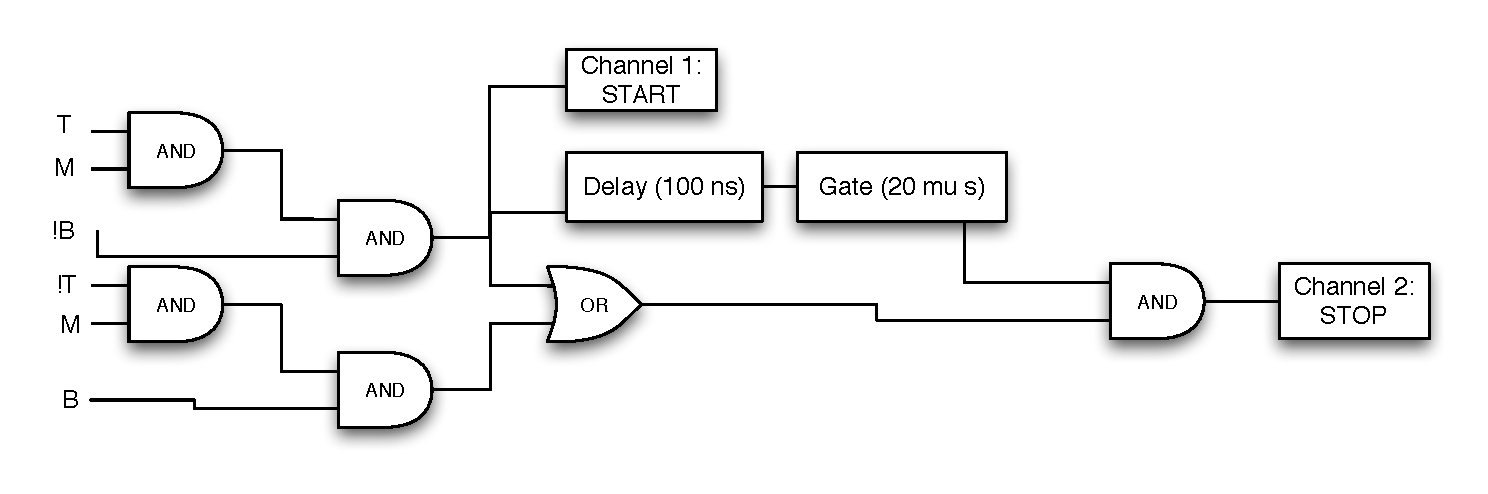
\includegraphics[height=50mm]{./figures/logicdiagram.eps}
\caption{Complete logic diagram for muon lifetime measurement}
\label{figure:logic}
\end{center}
\end{figure}


\subsection{Autocorrelator}
\label{autocorrelator}
In order to better study the effects of the photomultiplier false flashes, we used a Langley Ford Instruments Model 1096 Correlator to track the autocorrelation of the signal coming from each photomultiplier. The machine monitors at an input line for a signal, and records when another signal comes onto the same channel. We set it to record bins of $.1 \mu$s, up to a total of $8 \mu$s after the starting signal. Because the rate of muons coming into a scintillator is significantly smaller than this timescale, any autocorrelated signals could be strongly assumed to be false flashes (indeed, if there were extra muons coming in during this window, we would expect an even distribution over all times, but we did not see this). The results were normalized by dividing by the total number of signals detected over the run period.

\subsection{Measurements}
\label{measurements}
To make measurements, a LabView program takes data from an oscilloscope over a GPIB connection. For the lifetime experiment, the oscilloscope is set to trigger on a stop event, and the program measures the difference in time between the beginnings of the start and stop pulses, on channel 1 and 2 of the oscilloscope respectively. For the mass experiment, the scope is set to monitor for a trigger on channel 2 (a logic pulse indicating the required condition) and to monitor the height of pulses on channel 1 (the actual output from the photomultiplier).

%Results and Discussion body
%Created MS 1-30

\section{Results and Discussion}\label{results and discussion}

\subsection{Determination of Muon Lifetime}\label{determination of muon lifetime}

By constructing the logic pathway discussed in the previous section,
we can determine when a muon comes to rest in the middle scintillator
and correspondingly produce a START signal. Likewise, we can determine when the stopped muon decays by observing
the production of an electron with downward velocity, producing a STOP signal.  By observing the
duration between START and STOP signals, we are able to measure
the time it takes for a stopped muon to decay.  Essentially this time
is the lifetime of an individual muon.\footnote{The proper time
experienced during its time of flight before being stopped in the
scintillator blah bah}

This time data was measured and recorded over roughly a six day period
during which nearly $15000$ events were recorded.  To analyze this
data, we binned the time data to create a histogram shown in Figure~\ref{fig:muondecay} which measures number of events versus lifetime.
The binwidths were chosen to be $200 ns$. A good binwidth for data is given by the Freedman-Diaconis' choice,\footnote{ref}

\begin{equation}
\label{eq:binwidth}
h=2\frac{IQR}{N^{1/3}}
\end{equation}

where $h$ is the number of bins, $IQR$ is the interquartile range, and $N$ is the number data points in the set.  According to this formula, the optimal binwidth for our data is $227 ns$.  Because there does not exist a formula for optimal binwidth (the goodness of a specific binwidth is dependent upon the distribution of the data), the comparable binwidth of $200 ns$ is a valid, much more convenient choice. 



\begin{figure}[htbp]
\begin{center}
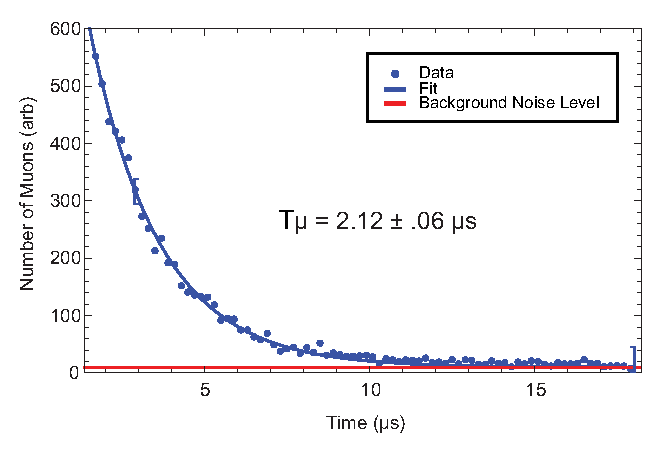
\includegraphics[height=70mm]{./figures/muon_decay.eps}
\caption{A histogram of muon lifetimes. The lifetimes follow exponential decay to some background noise level.  The data was fit using 2-parameter nonlinear regression using $\sqrt{N}$ weighting and excluding the first $2.0 \mu s$.  The fit has an $r^{2}$ value of $.996$ and produces a $\tau_{\mu}$ of $2.12 \pm .10 \mu s$.}
\label{fig:muondecay}
\end{center}
\end{figure}

 As a decay process with some time time constant, $\tau_{\mu}$, we
would expect the data to be modeled by the exponential decay of Equation
(4).  However because there is background noise recorded by our
scintillator the data is modeled by

\begin{equation}
\label{eq:fitdecay}
N(t) = N_{0} e^{-t/\tau_{\mu}}+b
\end{equation}

where $b$ is the constant background noise level measured by the scintillator. 

To determine the muon mean lifetime, $\tau_{\mu}$, we then fit the
data to Equation~\eqref{eq:fitdecay}.  Fitting involved three major processes: the
determination of the background noise level, $b$, determination of the
fitting range, and finally the determination of the muon mean lifetime
through using a 2-parameter nonlinear regression test based on Equation~\eqref{eq:fitdecay}.

To determine the noise background, a linear regression test was used.
We created an algorithm which iteratively tested increasingly large
portions of the tail end data from Figure~\ref{fig:muondecay} until we detected a
slight correlation ($p$-value $\leq .1$) between the points.  We took
this portion of noncorrelated tail end data to be the result of
background noise measured by the scintillator.  Accordingly, the mean
value of this subset was taken to be the background noise level,
$b$. From our data we determined the background noise level to be 10
events.

Determining the range over which we would fit the data to our model
was a crucial step in determining the mean lifetime of muons.  We
determined that the chance of data corruption increased for smaller
time values due to several uncontrollable systematic
limitations.\footnote{These limitations will be discussed in the
Blah.3.1} Likewise, we found that the goodness of our fit worsened as
we excluded an increasing amount of front end data points (most likely
due to the exclusion emphasizing the background noise dominating the
tail end data).  Resultantly, we determined that there existed an
optimal range over which to fit.  This range included data with time
values $t \geq t_{c}$, where $t_{c}$ is the cutoff time.  All data
points before and including $t_{c}$ were excluded from the fitting
process.  To determine $t_{c}$, we created an algorithm which
iteratively fit the data with increasing $t_{c}$ using a 2-parameter
nonlinear regression test.  For each fit, the $\tau_{\mu}$ and the
associated $r^{2}$ value were computed for $t_{c}\leq 5\mu s$.  These
results are shown in Figure~\ref{fig:rsq}.  We wanted $t_{c}$ to be a
value which corresponded to an $r^{2} \geq .995$ and a region of
minimally fluctuating $\tau_{\mu}$.  Observing the Figs, we decided
that ${.4\mu s \leq t_{c}\leq 2.0}$ was an adequate range for $t_{c}$.
Because data for smaller time values were more likely to be corrupted,
we ultimately chose our cutoff time to be $2.0 \mu s$.


\begin{figure}[htbp]
\begin{center}
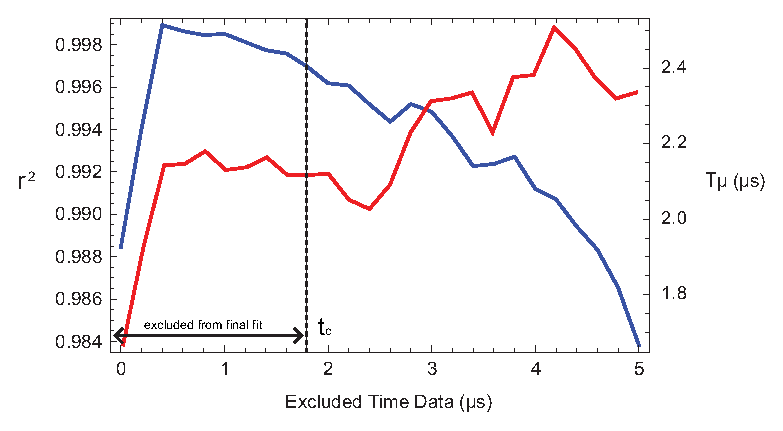
\includegraphics[height=60mm]{./figures/lifetime_fit_param.eps}
\caption{This plot shows the effect of excluding data up to some cutoff time $t_{c}$ from the fitting process.  We chose $t_{c}$ to be $2.0 \mu s$ because it produced a value for $\tau{\mu}$ that was in a range of relative stability and because it produced a fit with an $r^{2}$ value $> .995$ as seen above.}
\label{fig:rsq}
\end{center}
\end{figure}

Excluding all points prior to and including $t_{c}$, we were able to determine $\tau_{\mu}$ to be $2.12 \pm .16 \mu s$ with 95\% confidence.  This value deviates from the accepted value, $2.20\mu s$, by $3.6\%$.  However our $7.6\%$ error includes the accepted value.






\subsection{Determination of Muon Mass}\label{determination of muon mass}

By measuring the heights of pulses produced by PMT flashes, we are
able to ultimately determine the muon mass.  As discussed in Section
\ref{Muon Mass}, we can determine this mass by observing the electron cutoff energy, $E_{e}^{max}$. In order to measure electron energy in general
we first calibrated the PMT pulse height to the energy deposited in
the scintillator as discussed in Section \ref{Energy Calibration}. This calibration
was done by measuring the pulse heights of muon which passed through
all three scintillator panels.  More $50000$ events were observed in
roughly four hours of data aquisition.  The distribution of binned
pulse heights is shown in Figure~\ref{fig:pulseheights}(a).  As previously stated, the
maximum, or the mode, of this distribution corresponds to a minimum of
the BB equation (see Appendix).  From this we determined that a pulse
height $V_{\mu} = 9.8\pm.5 \times 10^{-2} V$ corresponds to a $\frac{dE}{dx}= 1.85\pm.10 MeV
g^{-1} cm^{2}$.  Knowing both the density and the thickness of the
scintillator panels to be $2.5\pm.2$ and $1.08\pm.09 g cm^{-3}$ respectively, we can determine
the actual scale between pulse height and deposited energy.  Taking
this scale to be approximately linear in this regime, we found that
$1V$ produced by the PMTs as measured by an oscilloscope, maps to an
energy of $51.3 \pm 8.3 MeV$.



\begin{figure}[htbp]
\begin{center}
\subfigure[Histogram of muon pulse heights]{\label{fig:edge-a}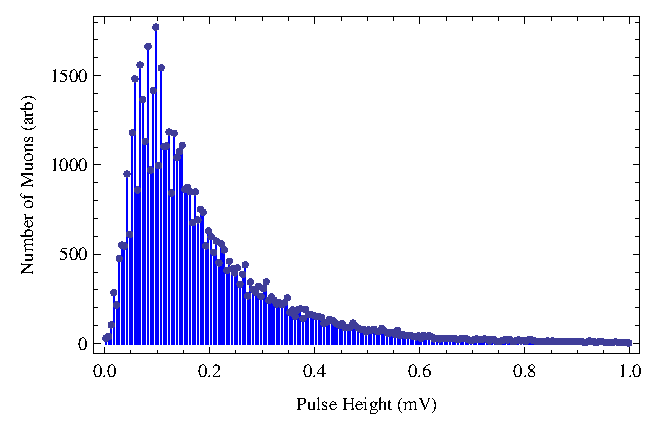
\includegraphics[height=52mm]{figures/Muon_Pulse_Height.eps}}
\hspace{-1mm}
\vspace{-2mm}
\subfigure[Histogram of electron pulse heights]{\label{fig:edge-b}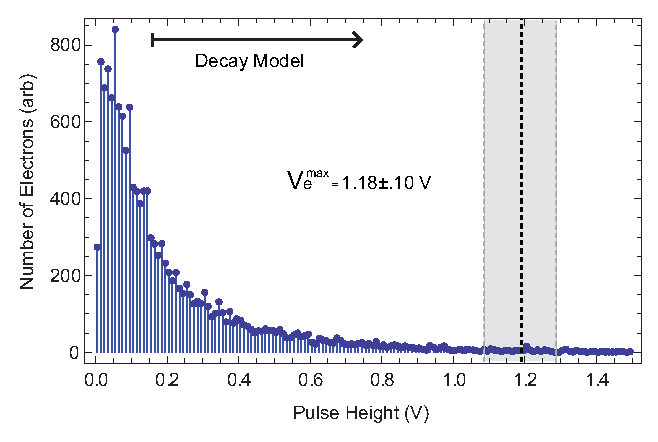
\includegraphics[height=52mm]{figures/Electron_Energy_Cutoff.eps}}
\vspace{-2mm}
\caption{These raw pulse heights produced by the PMTs correspond to muon and electron energies deposited in the scintillators.  Data from (a) is used to calibrate a scale from pulse height (measured in $V$) to energy (measured in MeV).  Data from (b) was used to determine the electron cutoff energy.  Together information from both plots were used to calculate the muon mass.}
\label{fig:pulseheights}
\end{center}
\end{figure}


By observing the pulse heights produced by PMT flashes from the middle
scintillator that correspond to STOP pulses, we then measured the
energy deposited by electrons produced from muon decay.  This data was
recorded for roughly five days and included nearly $7000$ events.  The
distribution of binned electron pulse heights, $V_{e}$, is shown in
Figure~\ref{fig:pulseheights}(b).  As noted in Section 2.3, the shape of this energy
distribution is determined by the kinematics of the muon decay.  Most
importantly, the energy cutoff (the point at which the distribution
decays to zero) occurs at roughly one-half the mass of the decayed
muon.




To determine the energy cutoff of the distribution in Figure~\ref{fig:pulseheights}(b), we
used a fitting algorithm.  First we assumed that after some pulse
height, the distribution could be approximately modeled by an
exponential decay.  To determine this value we did an $r^{2}$ analysis
of multiple fits to using 2-parameter nonlinear regression in which we
excluded an increasingly large range of low pulse heights points
beginning at $V_{e}=0$.  In these fits we weighted each data point by
$\sqrt{N_{e}}$, where $N_{e}$ is the number of electrons in some pulse
height bin.  We determined that the smallest exclusion range to
produce a fit with $r^{2}\geq.99$ was the exclusion range $0 V \leq
V_{e}\leq .1 V$.  We were then able to compute the model for the
decay distributions decay as $V_{e}$ approached the cutoff energy.
This model approximated the number of electrons one would expect to
see (relative to the number of events observed, which was nearly 7000)
for some $V_{e}$ .

The model for the distribution's decay was then used to determine
$E_{e}^{max}$ by finding the scope voltage at which the interval
$N_{e}\pm \delta N_{e}$ ($1-\sigma$ error bars) was completely below
$1$.  Because $N_{e}$ is a discrete value being modeled by exponential
decay, we claim that an $N_{e} \leq 1$ essentially corresponds to no
events.  Therefore we take this $V_{e}$, found to be $1.18\pm.10 V$,
to be $V_{e}^{max}$. We take all subsequent nonzero values of $N_{e}$
to be background noise produced by PMT false flashes.  Converting from
$V_{e}^{max}$, we find that $E_{e}^{max}=60.8 \pm 11.1 MeV$.  Based on
the kinematics of the muon decay we determined that this cutoff energy
implies a muon mass of $m_{\mu} = 122 \pm 22 MeV/c^{2}$.  This
value deviates from the accepted value, $105.66 MeV/c^{2}$, by $13.1\%$.
However our $18.2\%$ error includes the accepted value.

\subsection{Determination of Weak Force Coupling Constant}\label{determination of weak force coupling constant}

Having determined the parameters for both the muon mean lifetime, $\tau_{\mu}$, and the muon mass, $m_{\mu}$ we can calculate the value for $G_{F}$ using Equation (7). Ultimately, from our results we calculate that $G_{F}=blah \pm blah$.  This value deviates from the accepted value, $blah$, by $blah\%$. However our $blah\%$ error includes this accepted value.

Our calculation of $G_F$ is by no means a precision measurement.  Although certain aspects of this experiment have relatively low error ($<8\%$), such as the measurement of $\tau_{\mu}$, ultimately the overwhelming error associated with the energy calibration prevented a more precise measurement of $G_F$.


\end{document}







